% https://www.ctan.org/tex-archive/macros/latex/contrib/logicproof?lang=en
% https://en.wikibooks.org/wiki/LaTeX/Installing_Extra_Packages
% latex logicproof.ins
% latex logicproof.dtx
% mv logicproof.sty ~/texmf/tex/latex/logicproof/
% cd ~
% texhash texmf


\documentclass[12pt, a4paper]{article} %mostra o tipo do documento
\setlength{\topmargin}{-.5in}
\setlength{\textheight}{9in}
\setlength{\textwidth}{6.3in}
\setlength{\oddsidemargin}{-.125in}
\setlength{\evensidemargin}{-.125in}
\usepackage[brazil]{babel} % permite escrever em português
\usepackage[utf8]{inputenc}
\usepackage[T1]{fontenc} % define a fonte das letras
\usepackage{amsmath, amssymb, amsthm, amsfonts} % permite fazer textos matemáticos
\usepackage{float} % permite mover tabelas e figuras para qualquer ponto da página
\usepackage{graphicx} % permite colocar imagens no documento
\usepackage{color} % permite colorir o texto
\usepackage{listings}
\usepackage{logicproof}

\newcommand\then{\rightarrow}
\newcommand\liff{\leftrightarrow}

\title{\textbf{Lista 1 - MAC444}}
\date{}
\author{\textbf{João Gabriel Basi - $\text{N}^\circ$ USP: 9793801}}

\begin{document}
\maketitle
\begin{enumerate}
\item[\textbf{1.}]
\begin{enumerate}
\item[\textbf{a)}]
$D = \{a, b, c\}$\\
$I[P] = \{(a, b), (b, a)\}$\\
$I[a] = c$\\
$I[b] = a$\\

\item[\textbf{b)}]
$D = \{a, b, c\}$\\
$I[P] = \{(a, a), (b, b), (a, b), (b, a)\}$\\
$I[a] = c$\\
$I[b] = a$\\

\item[\textbf{c)}]
$D = \{a, b\}$\\
$I[P] = \{(a, a), (b, b), (a, b)\}$\\
$I[a] = a$\\
$I[b] = a$\\
\end{enumerate}

\item[\textbf{2.}]
\begin{enumerate}
\item[\textbf{a)}]
E(x): x é esquiador\\
A(x): x é alpinista\\
N(x): x gosta de neve\\
C(x): x gosta de chuva\\[0.4cm]
$D = \{\text{Tony}, \text{Mike}, \text{John}\}$
\begin{itemize}
\item $E(x) \lor A(x)$
\item $\lnot A(x) \lor \lnot C(x)$
\item $N(x) \lor \lnot E(x)$
\item $\lnot C(\text{Mike}) \lor \lnot C(\text{Tony})$
\item $C(\text{Mike}) \lor C(\text{Tony})$
\item $\lnot N(\text{Mike}) \lor \lnot N(\text{Tony})$
\item $N(\text{Mike}) \lor N(\text{Tony})$
\item $C(\text{Tony})$
\item $N(\text{Tony})$\\[2cm]
\end{itemize}

\item[\textbf{b)}]
Sabendo que $(x \lor y) \land (\lnot x \lor z) \vdash (y \land z)$ (regra da
resolução), temos:\\
$\text{KB} \vdash \exists x(A(x) \land \lnot E(x))$
\begin{logicproof}{1}
E(x) \lor A(x)\\
\lnot A(x) \lor \lnot C(x)\\
N(x) \lor \lnot E(x)\\
\lnot C(\text{Mike}) \lor \lnot C(\text{Tony})\\
C(\text{Mike}) \lor C(\text{Tony})\\
\lnot N(\text{Mike}) \lor \lnot N(\text{Tony})\\
N(\text{Mike}) \lor N(\text{Tony})\\
C(\text{Tony})\\
N(\text{Tony})\\
\begin{subproof}
\lnot A(x) \lor E(x) & suposição\\
E(x) & 1,10 resolução\\
N(x) & 3,11 resolução\\
N(\text{Mike}) & 12 x/Mike\\
\lnot N(\text{Tony}) & 7,13 resolução\\
\bot & 9,14 $\bot_i$
\end{subproof}
\exists x(A(x) \land \lnot E(x)) & 10-15 $\exists_i$
\end{logicproof}

\item[\textbf{c)}]

\item[\textbf{d)}]
.\\
\begin{center}
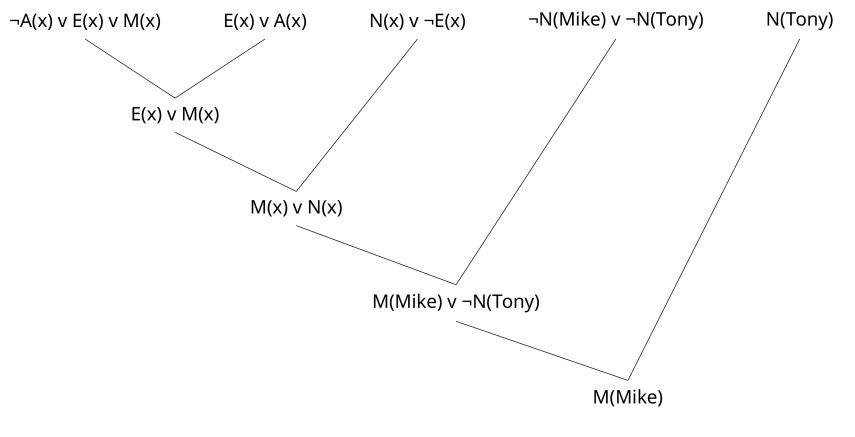
\includegraphics[scale=0.6]{tree.jpg}
\end{center}

\end{enumerate}
\end{enumerate}
\end{document}
